% Chapter 1

\chapter{Deep Learning and Tomographic Image Reconstruction} % Main chapter title

\label{Chapter2} % For referencing the chapter elsewhere, use \ref{Chapter1} 

%----------------------------------------------------------------------------------------
The impact of deep learning has been immense over the last few years in the field of medical imaging (\cite{litjens2017survey, greenspan2016guest}). Medical image reconstruction has also benefited hugely from the various advances in neural network architectures \cite{wang2020deep,yedder2021deep,reader2020deep}. In the specific case of \ac{CT} image reconstruction, there has been active interest in sparse-view and low-dose reconstruction scenarios. While with \ac{PET} reconstruction on the other hand, low-dose imaging and total body imaging have been on the forefront. In both cases, obtaining high quality reconstructed images is a challenging task. Many established model-based iterative methods account for the low-dose and sparse-view settings to remove artifacts and noise from the reconstruction (\cite{nuyts1998iterative,Elbakri2002,liu2013total}). However, these methods require the knowledge of noise and artifacts statistics and generally have longer reconstruction times \cite{kim2014combining}. Deep learning-based methods on the other hand are claimed to achieve reconstructed images with quality on par with iterative techniques and in a much shorter time frame \cite{leuschner2021quantitative}. In this work, the focus has been on \ac{CT} and \ac{PET} image reconstruction. 
Image reconstruction corresponds to the task of mapping raw projection data retrieved from the detector to image domain data. As depicted in Fig~\ref{fig:dl}, one can broadly identify three different categories of approaches for the implementation of deep learning within the framework of medical image reconstruction:
\begin{itemize}
	\item[(i)] methods that use deep learning as an image processing step that improves the quality of the raw data and/or the reconstructed image (\cite{gong2018pet, maier2018deep}); 
	\item[(ii)] methods that embed deep-learning image processing techniques in the iterative reconstruction framework to accelerate convergence or to improve image quality (\cite{xie2019generative,kim2018penalized,gong2019iterative});
	\item[(iii)] direct reconstruction with deep learning alone without any use of traditional reconstruction methods  (\cite{whiteley2019direct,zhu2018image,haeggstroem2018deeprec}).
\end{itemize}

\begin{figure}[!htbp]
	\centering
	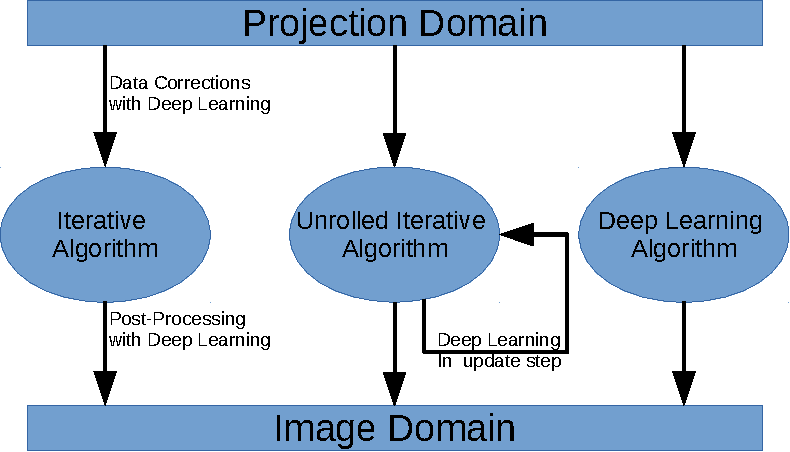
\includegraphics[width=0.8\linewidth]{./Figures/dl_mi.pdf}
	\caption{Deep Learning in Medical Image Reconstruction}
	\label{fig:dl}
\end{figure}


Each of these categories are discussed along with reference to existing state of the art methods for \ac{CT} and \ac{PET} image reconstruction in this chapter. 

\section{Data Corrections or Post-processing}

The use of deep learning for the development of either data corrections or post-reconstruction  image based approaches has shown potential to improve the quality of reconstructed images. While it is possible to train a \ac{CNN} to regress directly from the measurement (raw data) domain to the image domain, the use of \ac{CNN} entirely in one particular domain makes it fast and relatively easy to implement. The motivation behind using deep learning architectures for these processing task is the extremely well documented performance in denoising and super resolution tasks. Data corrections involve improving the measurement data either though denoising or finding missing projection angle data. Post-processing in the image domain on the other hand consists of improving images reconstructed with standard reconstruction methods. 


An example of data corrections by improving the raw data through scatter correction is proposed in \cite{maier2018deep}. In this work a modified U-Net is used to estimate scatter and correct the raw data in order to improve \ac{CT} images. Sinogram repair is proposed by \cite{whiteley2019cnn}, where a \ac{CNN} is utilized to predict missing projection data for total body \ac{PET} image reconstruction. The repaired sinograms eventually improve image reconstruction by standard methods. In \ac{CT} imaging too missing projection data in sparse-view setting is estimated. An example in this regard is proposed in \cite{lee2018deep}, where the authors use U-Net to map sparse-view sinograms to full-view sinograms and then reconstruct the images using \ac{FBP}. 



Denoising the reconstructed \ac{PET} images with a deep convolutional network was done in \cite{gong2018pet}. The authors used perceptual loss along with \ac{MSE} to preserve qualitative and quantitative accuracy of the reconstructed images. The network was initially trained on simulated data and then fine-tuned on real patient data. The authors in \cite{jin2017deep} use U-Net with a residual connection for denoising and artefact removal in the sparse-view estimate, while the work in \cite{zhang2018sparse} uses DenseNet with deconvolution for the same purpose. It is interesting to note that the networks have an encoder-decoder structure, wherein the encoder finds a compact representation of the input domain and the decoder learns to map this representation to the target domain. The dimensions of the input are reduced through the encoder as we go deeper into the layers. On the other hand, each of the decoder layers samples up these feature maps to eventually arrive at the output dimensions. 



\section{Unrolled Iterative Methods}

Despite resulting in an improvement of the reconstructed output, the above mentioned methods do not directly intervene with the reconstruction process. This can be done using the two distinct frameworks (ii) and (iii). The first one involves the incorporation of a deep neural network into an unrolled iterative algorithm where a trained neural network accelerates the convergence by improving the intermediate estimates in the iterations (\cite{gong2019iterative,xie2019generative,kim2018penalized}). The hybrid methodology of unrolled iterative networks combines model-based and neural network approaches exploring the benefits of both methods. 
The paper by Gong et al. used a modified U-Net to represent images within the iterative reconstruction framework for \ac{PET} images. The deep learning architecture was trained on low-dose reconstructed images as input and high-dose reconstructed images as the output. The work by Xie et al. further extended this work by replacing the U-Net with a \ac{GAN} for image representation within the iterative framework. Kim et al incorporated a trained denoising convolutional neural network (DnCNN) along with a novel local linear fitting function into the iterative algorithm. The DnCNN which is trained on data with multiple noise levels improves the image estimate at each iteration. They used simulated and real patient data in their study. In \cite{gupta2018cnn}, a U-Net is used to encode the prior, i.e., to project the current estimate to the prior image set while gradient descent enforces measurement consistency. Neural networks can be also used to replace traditional operators in optimization strategies as shown by \cite{adler2018learned}. The reconstruction using these hybrid methods can be computationally expensive since it requires running an optimization procedure at test time.

\section{Direct Reconstruction with Deep Learning}

An alternative approach is using deep learning-based methods to directly map from projection to image space. Essentially neural network can be modeled to approximately learn  the inverse mapping from measurement($y$) to image ($x$). As represented in Fig~\ref{fig:direct}, a neural network ($F$) with parameters ($\theta$) can be represented as:

\begin{equation}\label{eq:direct}
x=\boldsymbol{F}_{\widehat{\boldsymbol{\theta}}} \boldsymbol{y}
\end{equation}

The challenge in this approach is the management of data and the number of parameters required for learning the mapping. Due to these challenges, this approach has been less explored compared to the two approaches discussed above. 


\begin{figure}[!htbp]
	\centering
	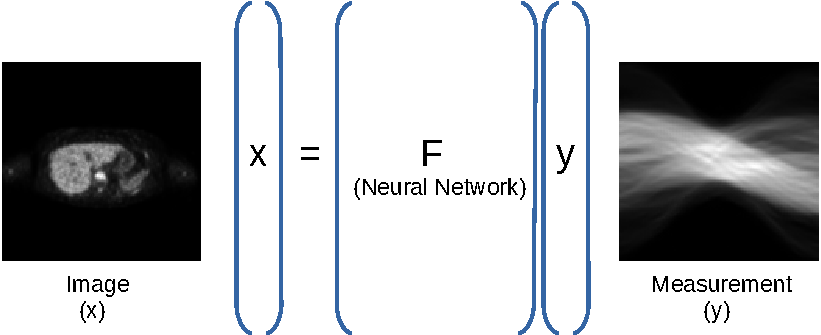
\includegraphics[width=0.8\linewidth]{./Figures/direct-crop.pdf}
	\caption{Direct image reconstruction with deep learning}
	\label{fig:direct}
\end{figure}

The deep learning architecture proposed by Zhu et al.~\cite{zhu2018image} called AUTOMAP uses \ac{FC} layers (which encode the raw data information) followed with convolutional layers.
The first three layers in this architecture are \ac{FC} layers with dimensions $2n^2$,$n^2$ and $n^2$ respectively where $n\times{}n$ is the dimension of the input image. The AUTOMAP requires the estimation of a huge number of parameters which makes it computationally intensive. Although initially developed for \ac{MRI}, AUTOMAP has been claimed to work on other imaging modalities too. Brain images encoded into sensor-domain sampling strategies with varying levels of additive white Gaussian noise were reconstructed with AUTOMAP.  Within the same concept of using \ac{FC} layers' architectures a three stage image reconstruction pipeline called DirectPET has been proposed to reduce associated computational issues  \cite{whiteley2019direct}. The first stage down-samples the sinogram data, following which a unique Radon transform layer encodes the transformation from sinogram to image space. Finally the estimated image is improved using a super resolution block. This work was applied to full body \ac{PET} images and remains the only approach that can reconstruct multiple slices simultaneously (up to 16 images). DeepPET is another approach implemented on simulated images using encoder-decoder architecture based on the neural network proposed by the visual geometric group \cite{haeggstroem2018deeprec}. Using realistic simulated data, they demonstrated a network that could reconstruct images faster, and with an image quality (in terms of root mean squared error) comparable to that of conventional iterative reconstruction techniques.  


In \cite{li2019learning} the authors proposed an architecture termed iCT-Net  consisting of $12$ layers that are a combination of convolutions and modified fully-connected layers. The $12$ layers are separated into segments and are trained separately before being combined for end-to-end training. To reduce the number of parameters in learning the mapping for full resolution \ac{CT} reconstruction, \cite{fu2019hierarchical} proposed a breakdown of the problem into smaller fragments that can be mapped onto a hierarchical network architecture. The approach proposed in \cite{ye2018deep} converts the sinogram data into a stack of back projections for each angle, which are then fed into a \ac{CNN}. The spatial in-variance of the \ac{CNN} is exploited to learn the mapping from these single view stacked back projections onto reconstructed images. Currently, we observe that adversarial networks are increasingly used in scenarios with high-resolution images. In \cite{thaler2018sparse} a Wasserstein generative adversarial network \cite{arjovsky2017wasserstein} is proposed for sparse-view \ac{CT} image reconstruction. The authors used a combination of $L_1$ loss and adversarial loss to train their network. The generator in their work is a U-Net and the discriminator a typical classification \ac{CNN}. It is to be noted that the authors performed their experiments on down-sampled images of resolution $128\times 128$. Another methodology referred to as DUG-RECON \cite{kandarpa2020dug}, used a three-stage network to divide the image reconstruction problem into denoising, domain mapping and resolution improvement. They used a residual UNet for denoising the sinograms, then a double-UNet architecture to map the sinogram to image, and finally a super ResNet to improve image estimate. The approach was tested with both \ac{PET} and \ac{CT} data. 




